\documentclass[UTF-8]{article}


\usepackage{booktabs}
\usepackage{url}
\usepackage{cite}
\usepackage[version=4]{mhchem}
\usepackage{graphicx}
\usepackage{subfigure}
\usepackage[a4paper,top=2cm,bottom=2cm,right=3cm,left=3cm,marginparwidth=1.75cm]{geometry}
\usepackage{amsmath}
\usepackage{upgreek}
\usepackage{listings}



\title{Verify the Theory of Natural Selection}
\author{Yan Haoming}
\date{November 22, 2024\\November 29, 2024\\December 1, 2024}


\begin{document}
\maketitle
\section{Introduction}
In this experiment, we repeated the study on mutation by Luria,S. E. and Delbrück,M.\cite{paper}
The hypothesis (mutation hypothesis instead of acquired hereditary hypothesis) we tried to verified is exactly in accordance to the theory of natural selection, which inspired me to title the report in this way.

The difference between our experiment and the original work lies mainly in experimental material.
Specifically, we used yeast rather than bacteria.
Besides, I carried out the simulation of the process on my laptop by Python which is impossible in the year of 1943.
\section{Theory}
\subsection{Key Concepts}
\begin{figure}[h]
    \centering
    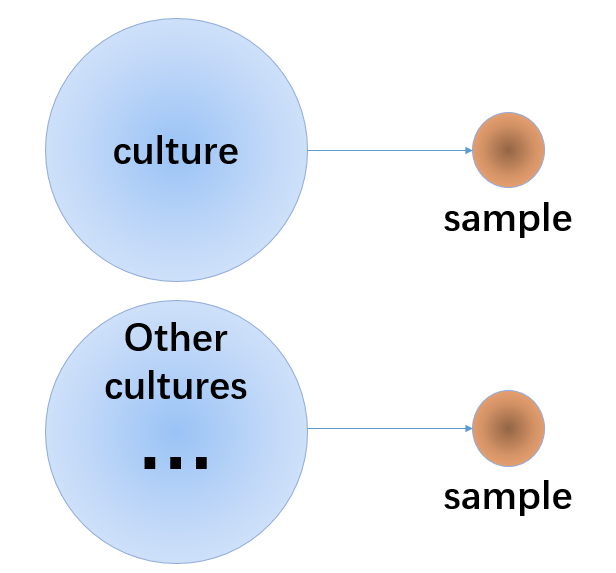
\includegraphics[width=0.5\linewidth]{../Figures/concept of culture and sample.png}
    \caption{Cultures and Samples}
    \label{Cultures and Samples}
\end{figure}
The concept of \textbf{culture} and \textbf{sample} should be distinguished clearly.
Each culture was cultured independently under the same condition serving as paralleled groups.
Samples were sampled out when spreading the plate representing the corresponding cultures.

Specifically speaking, cultures were grown in Multiwell Plate with 1 mL in each well.
Samples were 20 $\upmu$L ,which were sampled from each culture and spread onto to a solid plate.
\subsection{Meaning of Symbols}
To emphasis the time dependence of some variables, I add subscripts to them, which is slightly different from the original article.
\begin{itemize}
    \item $C$: number of similar \textbf{cultures} in our experiment.
    \item $t$: time in units of division cycles of the yeasts.
    \begin{itemize}
        \item thus the growth rate should be exactly 1, both for sensitive yeasts and resistant yeasts.
        \item $t_0$: a certain time, prior to which mutations were not likely to occur in any experimental \textbf{cultures}.
        Specifically speaking the $t_0$ satisfies:
        $$
        1=\text{Ex}(Cm_{t_0}))=\text{Ex}(aC(N_{t_0}-N_0))
        $$
    \end{itemize}
    \item $N_t$, \textit{observable}: number of yeasts in \textbf{a growing culture} at time $t$.
    \begin{itemize}
        \item $N_t-N_0$: increase in the number of yeasts.
        \item $N_0\ll N_t$, thus, $N_0\approx 0$ in the presence of $N_t$.
    \end{itemize}
    \item $\rho _t$: the \textbf{average} number of resistant yeasts present at time $t$, in one \textbf{culture}.
    \item $r_t$, \textit{observable}: the \textbf{likely average} number of resistant yeasts in a \textbf{culture} at time $t$, gotten from \textbf{limited number of samples}.
    \item $a$: mutation rate, namely, the chance of mutation per yeast per time unit.
    \item $m_t$: the \textbf{average} number of mutations at time $t$, in \textbf{a culture}.
    \item $p_0$: the fraction of cultures showing \textbf{no} mutation in a large series of similar cultures.


\end{itemize}
\begin{figure}[h]
    \centering
    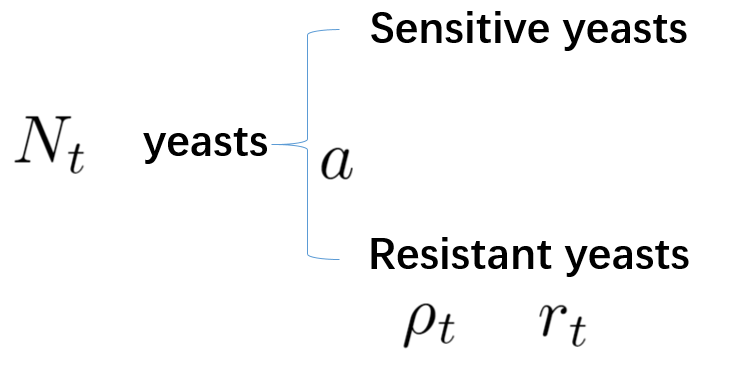
\includegraphics[width=0.5\linewidth]{../Figures/number of yeasts.png}
    \caption{Number of Yeasts Divides into Sensitive One and Resistant One}
    \label{number of yeasts}
\end{figure}
\subsection{Derivation of the Formulas}
\subsubsection{Acquired Hereditary Immunity Hypothesis}
\textit{Assumption: a fixed small chance for each yeast to survive an attack.}
\begin{align}
    \text{Number of resistant yeasts}&\sim\text{Binomial Distribution}\\
    &\sim\text{Poisson Distribution}
\end{align}
\begin{align}
    \text{Var}(r_t)&=\text{Ex}(r_t)=r_t\\
\end{align}

\subsubsection{Mutation Hypothesis}
\textit{Assumption: a fixed small chance per time unit for each yeast to undergo a mutation to resistance.}
\begin{align}
    \frac{dN_t}{dt}&=N_t\\
    N_t &=N_0e^t\\
    dm_t &=a dt N_t\\
    m_t &=a(N_t-N_0)
\end{align}
\begin{align}
    \text{Number of yeasts mutate during }dt&\sim\text{Poisson Distribution}
\end{align}
\begin{align}
    p_0&=e^{-m_t}\\
    \frac{d \rho _t}{dt}&=aN_t+\rho\\
    \text{assume: }\rho_0&=0\\
    \rho_t&=taN_t\\
    r_t&=(t-t_0)aN_t\\
    1&=aC(N_{t_0}-N_0)\approx aCN_{t_0}\\
    N_{t_0}&=N_te^{-(t-t_0)}\\
    t-t_0&=\ln(N_tCa)\\
    r_t&=aN_t\ln(N_tCa)
\end{align}
The following discussion is about \textbf{partial distribution}, defined as the distribution during a certain time interval from $t-\tau$ to $t-\tau+d\tau$ with $t$ fixed while $\tau$ as parameter:
\begin{align}
    \text{Ex}(dm_t)&=aN_{\tau}d\tau =aN_te^{-\tau}d \tau\\
    d\rho_t&=e^{\tau}dm_t\\
    \text{Ex}(d\rho_t)&=e^{\tau}\text{Ex}(dm_t)=aN_td\tau\\
    \text{Var}(d{\rho_t})&=e^{2\tau}\text{Var}(dm_t)=aN_te^{\tau}d\tau\\
\end{align}
To find the total distribution from partial distribution:
\begin{align}
    \text{Var}({\rho_t})&=\int_{0}^{t}\text{Var}({d\rho_t})d\tau\\
    &=aN_t(e^t-1)\\
    \text{Var}({r_t})&=\int_{0}^{t-t_0}\text{Var}({dr_t})d\tau\\
    &=aN_t(e^{t-t_0}-1)\\
    &\approx Ca^2N_t^2\\
    \frac{\text{Var}(r_t)}{r_t}&=\frac{CaN_t}{\ln(N_tCa)}\gg 1
\end{align}
\section{Calculating Procedure in Experiment}
\begin{itemize}
    \item observe the number of yeasts in a growing culture $N_t$ at time $t$.
    \item determine the number of resistant yeasts in each \textbf{sample}.
    \begin{itemize}
        \item this should be carried out by observing the number of colonies several days after inoculating.
    \end{itemize}
    \item calculate the number of resistant yeasts $r_t$ in each \textbf{culture}:
    $$
    r_t=\text{Ex}(r_t)=\frac{\text{volume of culture}}{\text{volume of samples}}\cdot \text{Ex}(r_{t\text{ sample}})
    $$
    \begin{itemize}
        \item $\text{volume of culture}=1$ mL, $\text{volume of samples}=20\ \upmu $L in our experiment.
    \end{itemize}
    \item evaluate the mutation rate $a$ by the following formula:
    $$
    r_t=\text{Ex}(r_t)=aN_t\ln(N_tCa)
    $$
    \item figure out the likely variance $\text{Var}(r_t)$:
    \begin{itemize}
        \item by mutation rate $a$ according to the theory:
        $$
        \text{Var}({r_t})\approx Ca^2N_t^2
        $$
        \item by statistical methods:
        
        $$
        \text{Var}(\tilde{r_{t \text{ sample}}})=\text{Var}(r_{t \text{ sample}})-\text{Var}(\text{sampling})
        $$

        $$
        \text{Var}(\text{sampling})\approx\text{Ex}(\text{sampling})=r_t
        $$
        $$
        \text{Var}({r_t})=\left( \frac{\text{volume of culture}}{\text{volume of samples}} \right)^2\cdot\text{Var}(\tilde{r_{t \text{ sample}}}) 
        $$
        Thus we calculate the modified statistical variance by:
        $$
        \text{Var}({r_t})=\left( \frac{\text{volume of culture}}{\text{volume of samples}} \right)^2\cdot(\text{Var}(r_{t \text{ sample}}) -\text{Ex}(r_{t \text{ sample}}))
        $$
        \item compare the ratio of variance and average to one (Poisson distribution in Acquired hereditary immunity hypothesis):
        $$
        \frac{\text{Var}(r_t)}{\text{Ex}(r_t)}
        $$
        both by the statistical method (just based on the final result) and by the theoretical method (based on the mutation rate $a$).
    \end{itemize}


\end{itemize}
\section{Materials and Experimental Procedure}
We adopted YNB, glucose, and Amino Acids to make the culture medium.
The pressure of selection was introduced by canavanine, which can distinguish the resistant yeasts from sensitive yeasts.

The following solutions were prepared.
\begin{itemize}
    \item 10x YNB 500 mL 
    \item 10x glucose 500 mL
    \item 10x Amino Acids 500 mL
    \item 10x Amino Acids without Arginine 500 mL
    \item 100x canavanine 100 mL
\end{itemize}

The detailed configuration of selective culture medium is shown below:
\begin{itemize}
    \item 10x YNB 100 mL 
    \item 10x glucose 100 mL
    \item 10x Amino Acids without Arginine 100 mL
    \item 100x canavanine 10 mL
\end{itemize}

And pour 25 mL mixture to one plate.

As for SD culture medium:
\begin{itemize}
    \item 10x YNB 100 mL 
    \item 10x glucose 100 mL
    \item 10x Amino Acids 100 mL
\end{itemize}

And pour 25 mL mixture to one plate in the same way.

We found out the proper concentration (approximately 100 yeasts/mL) by serial dilution.
And then added them to Deep-well Multiwell(96) Plate for culturing. After a week, spread the yeasts to solid culture medium. Three days later, stopping culturing and we counted the colonies in each drop in both experimental group and controlled group.

\section{Data Analysis}

\subsection{Calculate Sampling Variance}
\begin{figure}[h]
    \centering
    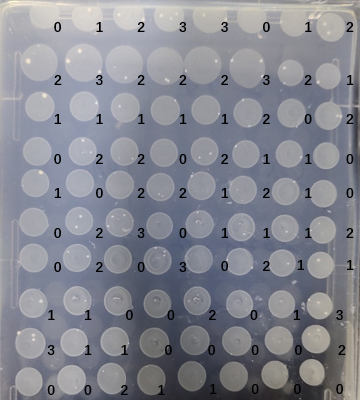
\includegraphics[width=0.5\linewidth]{../Figures/controlled group.png}
    \caption{Controlled Group}
    \label{controlled group}
\end{figure}
I firstly calculate the sampling (from culture to sample) variance by the controlled group as shown in Figure \ref{controlled group}.
In Table \ref{Statistics of Controlled Group}, I have shown the mean and variance of $r_{t \text{ sample}}$ .
The mean value is close to variance indicating the sampling process follow Poisson distribution.

It should be noted that unbiased estimator is adopted to estimate.

Frankly speaking we could get the final result even if without controlled group.
The role of controlled group is to confirm us that the randomness introduced by sampling follows Poisson Distribution.

$$
0.97=\text{Var}(\text{sampling})\approx\text{Ex}(\text{sampling})
$$

% Table
\begin{table}[h]
    \centering
    \begin{tabular}{|c|c|}\hline
        Mean $\bar {x}$ & 1.1625 \\ \hline
        Variance $S^2x$ & 0.9733\\ \hline
        Capacity & 80\\ \hline
    \end{tabular}
    \caption{Statistics of Controlled Group}
    \label{Statistics of Controlled Group}
\end{table}
\subsection{Number of Total Yeasts in Cultures}
\begin{table}[h]
    \centering
    \begin{tabular}{|c|c|c|}\hline
        Culture Number & Concentration (number per mL)& Number $N_t$ in a culture\\ \hline
        C1 & $6.67\times 10^7$ & $6.67\times 10^7$\\ \hline
        C4 & $1.38\times 10^6$ & $1.38\times 10^6$\\ \hline
        C7 & $1.41\times 10^6$ & $1.41\times 10^6$\\ \hline
        F12 & $4.57\times 10^7$ & $4.57\times 10^7$\\ \hline
        F9 & $1.79\times 10^8$ & $1.79\times 10^8$\\ \hline
        Mean & $5.88\times 10^7$ & $5.88\times 10^7$\\ \hline
    \end{tabular}
    \caption{Number of Yeasts in Cultures}
    \label{Number of Yeasts in Cultures}
\end{table}

To calculate mutation rate $a$ , we should first figure out the number of yeast in a culture, namely $N_t$.
Therefore we randomly selected five cultures from experimental group and counted the number of yeasts respectively before spreading to the plate (solid culture medium).

The results are shown in Table \ref{Number of Yeasts in Cultures}.
To be noted that the volume is exactly 1 mL per culture (deep well in the plate).


Finally taking the average number to be $N_t$ for further calculation.

$$
N_t=5.88\times 10^7
$$

\subsection{Number of Resistant Yeasts in Samples}
\begin{figure}[h]
    \centering
    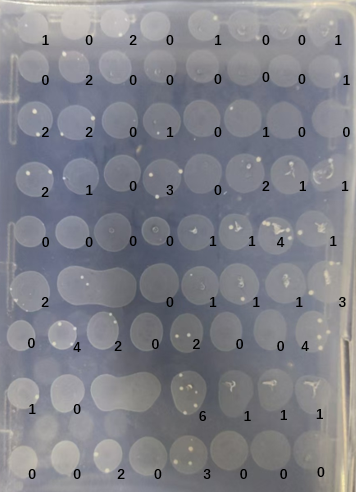
\includegraphics[width=0.5\linewidth]{../Figures/experimental group.png}
    \caption{Experimental Group}
    \label{experimental group}
\end{figure}
The critical statistics are gotten from experimental groups as shown in Figure \ref{experimental group} and Table \ref{Statistics of Experimental Group}.
Again, the mean value in experimental groups (0.97) is close to the variance of controlled group (0.9733, representing sampling variance), which demonstrate the correctness of our train of thought.

\begin{table}[h]
    \centering
    \begin{tabular}{|c|c|}\hline
        Mean $\bar {x}$ & 0.9706 \\ \hline
        Variance $S^2x$ & 1.5812\\ \hline
        Capacity & 68\\ \hline
    \end{tabular}
    \caption{Statistics of Experimental Group}
    \label{Statistics of Experimental Group}
\end{table}

\subsubsection{The Expectation Value}

\begin{align}
    \text{Ex}(r_{t\text{ sample}})&=0.97 \\
    \text{volume of culture}&=1 \text{ mL}\\
    \text{volume of samples}&=20\ \upmu\text{L}\\
    \text{Ex}(r_t)&=\frac{\text{volume of culture}}{\text{volume of samples}}\cdot \text{Ex}(r_{t\text{ sample}})\\
    &=\frac{1\times 10^3}{20}\times 0.97=48.5
\end{align}

\subsubsection{The Variance: By Statistical Methods}
\begin{align}
    \text{Var}(r_{t\text{ sample}})&=1.5812\\
    \text{Var}(\tilde{r_{t \text{ sample}}})&=\text{Var}(r_{t \text{ sample}})-\text{Var}(\text{sampling})\\
    \text{Var}(\text{sampling})&\approx\text{Ex}(\text{sampling})=r_t\\
    \text{Var}({r_t})&=\left( \frac{\text{volume of culture}}{\text{volume of samples}} \right)^2\cdot\text{Var}(\tilde{r_{t \text{ sample}}}) \\
    \text{Var}({r_t})&=\left( \frac{\text{volume of culture}}{\text{volume of samples}} \right)^2\cdot(\text{Var}(r_{t \text{ sample}}) -\text{Ex}(r_{t \text{ sample}}))\\
    &=\left(\frac{1\times 10^3}{20}\right)^2\times(1.5812-0.97)=1528
\end{align}
\subsection{Mutation Rate and Variance: By Theoretical Methods}
We can evaluate the mutation rate $a$ by the following formula:
\begin{align}
    C &= 68\\
    \text{Ex}(r_{t})&=48.5 \\
    N_t&=5.88\times 10^7\\
    r_t&=\text{Ex}(r_t)=aN_t\ln(N_tCa)  \\
    a&=1.32\times 10^{-7} 
\end{align}
Thus the corresponding variance is:
\begin{align}
    \text{Var}({r_t})&\approx Ca^2N_t^2\\
    &=4074
\end{align}

\subsection{Verification}
\subsubsection{By Statistical Methods}
$$
\frac{\text{Var}(r_t)}{\text{Ex}(r_t)}=\frac{1528}{48.5}=31.5 \gg 1
$$
\subsubsection{By Theoretical Methods (Based on Mutation Rate)}
$$
\frac{\text{Var}(r_t)}{\text{Ex}(r_t)}=\frac{4074}{48.5}=84 \gg 1
$$
\subsection{Conclusion}
$$
        \frac{\text{Var}(r_t)}{\text{Ex}(r_t)}\gg1
$$
From our experiment, it has been verified that, the ratio of variance to mean value is much greater than one, both by the statistical method (just based on the final result) and by the theoretical method (based on the mutation rate $a$).
Therefore, the acquired hereditary immunity hypothesis is wrong while the mutation hypothesis is more sensible.
\section{Simulation}
I wrote the computer program in the logic of each hypothesis to simulate the corresponding mechanisms.
After that, I calculated the statistics including mean value and variance to confirm the validity of former theoretical analysis.
\subsection{Acquired Hereditary Immunity Hypothesis}
\begin{figure}[h]
    \centering
    \subfigure[$N_t-t$]{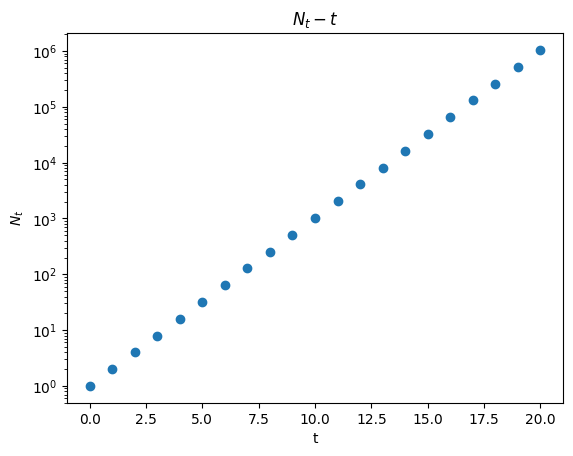
\includegraphics[width=0.45\linewidth]{../Figures/h1-nt-t.png}}
    \subfigure[Distribution of resistant yeasts in one culture]{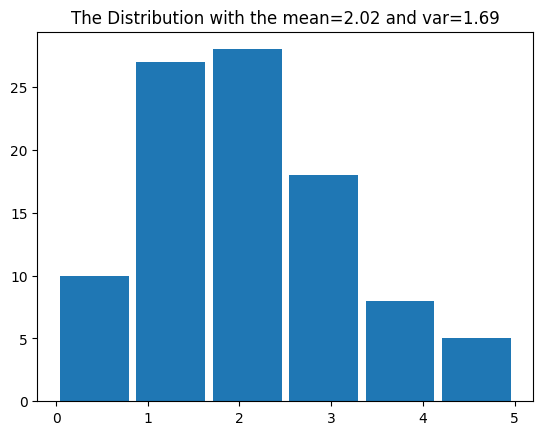
\includegraphics[width=0.45\linewidth]{../Figures/h1-dis.png}}
    \caption{Simulation on Acquired Hereditary Immunity Hypothesis}  
    \label{Simulation on Acquired Hereditary Immunity Hypothesis}
 \end{figure}
As we can see in Figure \ref{Simulation on Acquired Hereditary Immunity Hypothesis}, the mean value is close to variance.
\begin{align}
    \text{Ex}(r_t)&=2.02\\
    \text{Var}(r_t)&=1.69\\
    \frac{\text{Var}(r_t)}{\text{Ex}(r_t)}&=1.195\approx1
\end{align}

\subsection{Mutation Hypothesis}
\begin{figure}[h]
    \centering
    \subfigure[$N_t-t$]{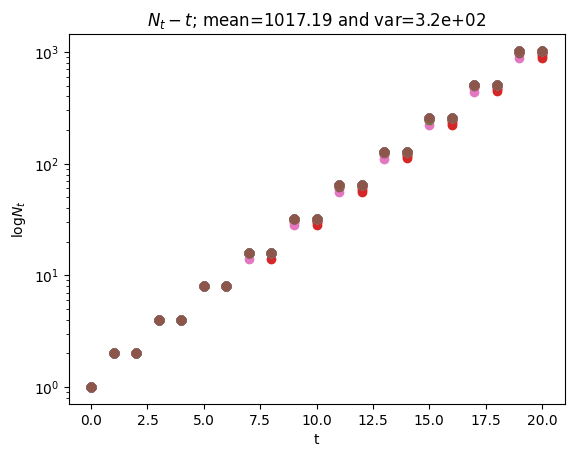
\includegraphics[width=0.45\linewidth]{../Figures/h2-nt-t.png}}
    \subfigure[$r_t-t$]{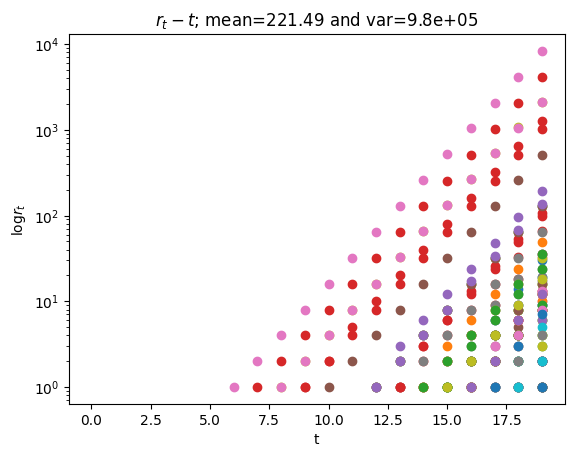
\includegraphics[width=0.45\linewidth]{../Figures/h2-rt-t.png}}
    \caption{Simulation on Mutation Hypothesis}  
    \label{Simulation on Mutation Hypothesis}
 \end{figure}
 As we can see in Figure \ref{Simulation on Mutation Hypothesis}, the variance is much greater than the mean value.
 \begin{align}
    \text{Ex}(r_t)&=221.49\\
    \text{Var}(r_t)&=9.8\times 10 ^5\\
    \frac{\text{Var}(r_t)}{\text{Ex}(r_t)}&=4.4\times 10^3\gg1
\end{align}

The bigger variance compared with acquired hereditary immunity hypothesis is very intuitive.
On the acquired hereditary immunity  hypothesis, the randomness is only introduced at the moment of selection or attack, \textbf{which happens only once}.
However, under the mutation hypothesis, the source of randomness is mutation .
There is mutation in each generation and therefore the \textbf{randomness will be accumulated}.
That is the nature of large variance.

\begin{figure}[h]
    \centering
    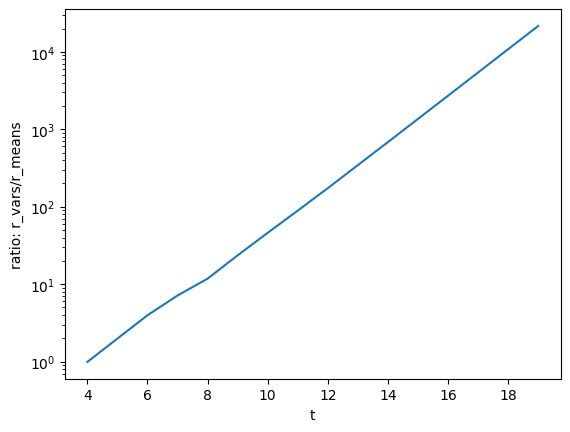
\includegraphics[width=0.4\linewidth]{../Figures/ration.png}
    \caption{Increasing Ratio with Respect to Time}
    \label{ratio-time}
\end{figure}

For the convenience of adjusting configuration of the simulation, I further analyzed the increasing trend of the ratio $\text{Var}/\text{Ex}$ as shown in Figure \ref{ratio-time}.

It can be clearly seen that that the ration of variance to mean value increase rapidly with time.

\newpage
\section{Conclusion}
In this experiment we verified the mutation hypothesis, in accordance with the theory of natural selection.
The simulation of the two different mechanisms helped me to grasp the nature of bigger randomness, while providing supporting evidence for our experiment.
Thanks for the instruction from teaching assistant.
\bibliographystyle{plain}
\bibliography{references}
\end{document}